\documentclass[10pt,twocolumn,letterpaper]{article}
\usepackage[margin=0.7in]{geometry}
\usepackage{cite,amsmath,amssymb,amsfonts,amsthm}
\newtheorem{theorem}{Theorem}
\newtheorem{proposition}[theorem]{Proposition}
\newtheorem{lemma}{Lemma}
\newtheorem{corollary}[theorem]{Corollary}
\usepackage{graphicx,textcomp,mathtools,booktabs,array,tabularx,calc,microtype,placeins,etoolbox,xurl}
\usepackage[hidelinks]{hyperref}
\urlstyle{same}
\newcommand{\PARstart}[2]{#1#2}
\newcommand{\EOD}{}
\setlength{\emergencystretch}{1em}
\setlength{\columnsep}{0.24in}
\renewcommand{\dbltopfraction}{0.9}
\setlength{\parskip}{0pt}
\begin{document}
\twocolumn[{\centering\Large\bfseries Physical Gradient Recovery and Stopping Guarantees for a Folded Stokes Parametrization\par}\vspace{0.6em}{\centering\small Hiroyasu Usami, Ayato Tsuboi, and Keisuke Hara\par Research draft, 22 October 2026\par}\vspace{1em}
\begin{minipage}{\textwidth}\small\textbf{Abstract.}
Small derivatives in a constraint-enforcing parametrization can coexist with a substantial physical objective gap. For the rational Stokes map, first derivatives lose one physical-gradient component at full polarization. We recover it from one signed radial curvature for any twice continuously differentiable objective, including nonstationary points with an unknown physical Hessian. Near the fold, mixed-scalar and vector-Hessian inverses give explicit derivative- and curvature-input error gains. For strongly convex physical objectives on the inner sheet with bounded intensity, a normalized head-gradient tolerance $\varepsilon$ and a radial lower-curvature tolerance $\nu$ yield an explicit objective-gap bound with sharp orders $\varepsilon^{4/3}+\nu^2$. Valid derivative-error budgets give sufficient stopping thresholds. An outward interval implementation for the nominal ideal quadratic certifies a gap at most $10^{-6}$ at 8\,861 of 9\,284 stored warm-start endpoints, using 52 scalar curvature evaluations. Controlled two-frame and noisy Fresnel fits exhibit fold-related inaccurate solver acceptance. Released observations reveal broader failures that the local fold gate misses. Coordinate repair corrects 249 of 295 inaccurate warm-start acceptances in a paired audit; standard physical fallback corrects the remaining 46. Direct physical solvers are cheaper in the tested implementation. Twenty shared-network fits contain no near-fold negative-curvature candidates at the saved checkpoints.
\end{minipage}\vspace{1.5em}
]
\section{Introduction}
\label{sec:intro}
\PARstart{S}{mall} derivatives of a constraint-enforcing output map can cause an optimizer to stop while the physical objective remains inaccurate. We study this problem for the rational Stokes parametrization, which represents physically admissible linear polarization. At full polarization, its first derivatives leave one physical-gradient component undetermined. One signed radial second derivative recovers that component, even at a nonstationary point with unknown physical Hessian. Figure~\ref{fig:principle} exhibits objectives with the same value, first head derivatives, and physical Hessian but different physical gradients; their radial second derivatives distinguish them.

Physicality-constrained Stokes estimation enforces an admissible polarization state \cite{hu,spc,psara}. Polarization also supplies cues for learned shape and inverse rendering \cite{ba,pandora}, with acquisition noise requiring separate evaluation \cite{polarns}. Smooth output maps offer one way to enforce constraints in differentiable models. Optimization layers \cite{optnet,cvxlayers} and constrained networks \cite{hardnet} make the differential information carried by such maps a relevant design question.

The rational ball map and its first derivative are established \cite[Sec.~V-B, (78)--(79)]{gcopter}. Smooth-lift theory describes how critical-point properties transfer through a parametrization \cite{lifts}; Hadamard parametrizations provide related stationary-point and strict-saddle correspondences \cite{hadamard}. Our question concerns the inverse information: which signed derivative values determine the physical gradient? Table~\ref{tab:priorart} relates the statements. The contribution is the explicit Stokes inverse and its sensitivity coefficients within this differential framework.

Proposition~\ref{prop:recovery} gives scalar and vector recovery formulas at the fold for any $C^2$ objective, without stationarity. Away from the fold, complete first derivatives already identify the gradient, but their radial inverse amplifies errors. Propositions~\ref{prop:mixed} and \ref{prop:localcurvature} correct second-order observations using, respectively, one physical-curvature scalar or one Hessian action. The corresponding error formulas identify which input causes each radial or tangential amplification. Corollary~\ref{cor:gap} then converts recovered gradients into a quadratic gap bound, with an exact tightness condition and the slack required at interior outputs.

Theorem~\ref{thm:uniformstopping} gives a uniform stopping bound for strongly convex physical objectives. On the inner sheet with bounded intensity, normalized first derivatives and a lower test on one radial curvature bound the gap by an explicit expression of order $\varepsilon^{4/3}+\nu^2$. The result holds throughout this domain, including points far from the optimum. Sharp examples, derivative-error budgets, and counterexamples specify its accuracy and scope. It builds on quantitative second-order transfer for squared-variable formulations \cite{dingwright} and the degenerate behavior described by known Kurdyka--\L{}ojasiewicz (KL) exponents for Hadamard models \cite{ouyang}. The Stokes specialization supplies explicit constants and uses a single curvature direction.

The observation sets in Table~\ref{tab:contract} are stipulated local information models. At a stationary fold, head derivatives alone classify a calibrated convex quadratic: the radial curvature is nonnegative at the constrained optimum and negative at a strict saddle, a stationary point with a negative head-Hessian eigenvalue. Away from the fold, the polarization Hessian block $H_{pp}=W_{pp}$ is fixed by the calibrated instrument and weighting, independently of the observations. Supplying that curvature therefore does not require prior knowledge of the gradient. When the full model and data are exposed, direct physical differentiation remains available and is included in the automatic differentiation (AD) benchmark.

The numerical evaluation tests the formulas on nonquadratic objectives, measures acquisition cost and finite-precision error on a common graph, and records near-fold curvature in 20 shared multilayer-perceptron (MLP) fits. Controlled two-frame fits and a noisy Fresnel-reflection sequence then test the diagnosis of inaccurate solver acceptance after a raw warm start. A fixed released-data audit includes both static observations and real bursts. It separates fold-related diagnosis from broader small-derivative failures, using cold starts, physical stopping bounds, and the direct cone optimum as controls. A follow-up on these known observations compares coordinate repair with cold restarting and physical projected gradient, retaining the stronger direct controls and the failures of switching alone. Continuous-flow geometry is kept separate from all measured discrete-solver behavior.

We develop diagnostics and conditional stopping guarantees for optimization through a Stokes output head. Within an existing fitting pipeline, the recovery formulas expose physical-gradient information and the gap bounds assess a solver endpoint. Table~\ref{tab:contract} specifies the derivative observations and physical-curvature inputs required by each route.

\begin{figure*}[!t]
\centering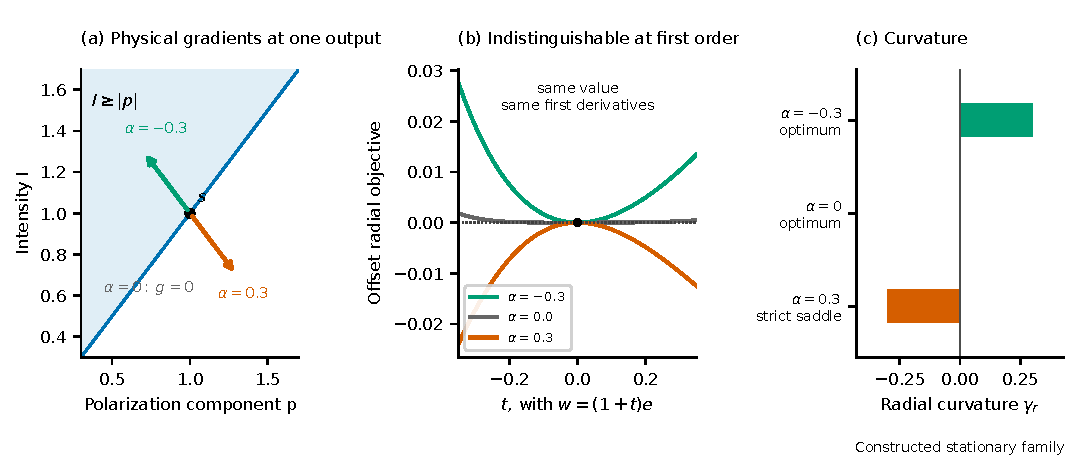
\includegraphics[width=\textwidth]{images/identifiability_principle.pdf}
\caption{Identical first-order information, different physical gradients. Fix $I=1$, $e=(1,0)$, $s=(1,e)$, the ideal four-analyzer metric $W=\operatorname{diag}(1,1/2,1/2)$, and $z_\alpha=s-\alpha W^{-1}n$, $n=(-1,e)$ for $\alpha=-0.3,0,0.3$. The objectives are $f_\alpha(u)=\tfrac12\|u-z_\alpha\|_W^2+c_\alpha$, with $c_\alpha$ chosen so that $f_\alpha(s)=0$. (a) The physical gradients $g_\alpha=\alpha n$ differ at the same output. (b) The objectives have identical value, zero first head derivatives, and the same physical Hessian. Their radial slices separate at second order. (c) In this stationary family, $\gamma_r=c_r=-I\alpha$ distinguishes two constrained optima from a strict saddle. The general gradient-recovery identity also holds without stationarity.}
\label{fig:principle}
\end{figure*}


\begin{table*}[!t]
\caption{Observations and supplied curvature. Recovery uses any $C^2$ objective with known geometry, $I>0$, $r>0$. The gap row additionally assumes a fixed calibrated quadratic with $W\succ0$.}
\label{tab:contract}
\centering\small\renewcommand{\arraystretch}{1.13}
\begin{tabularx}{\textwidth}{@{}p{.18\textwidth}p{.22\textwidth}p{.24\textwidth}X@{}}\toprule
Route & Head observations & Physical-curvature input & Result and domain\\\midrule
Fold scalar & $b,j,c_r$ & None & Full gradient, \eqref{eq:scalarrecovery}; $r=1$\\
First-order inverse & $b_r,j_r$ & None & Full gradient, \eqref{eq:firstinverse}; $r\ne1$\\
Mixed scalar & $b_r,P_\perp j_r,c_r$ & Scalar $h_{rr}=e^{\mathsf T}H_{pp}e$ & \eqref{eq:mixedrecovery}; $r\ne\sqrt3$; curvature cancels at $r=1$\\
Vector HVP & $b_r,v_r$ & Action $h_p=H_{pp}e$ & \eqref{eq:correctedrecovery}; $r\ne\sqrt3$; curvature cancels at $r=1$\\
Quadratic gap & Recovered gradient & Fixed metric $W$ & Corollary~\ref{cor:gap}; supporting normal and interior slack\\\bottomrule
\end{tabularx}
\end{table*}

\begin{table*}[!t]
\caption{Relation to prior results. Locators for \cite{lifts} refer to arXiv:2207.03512v5.}
\label{tab:priorart}
\centering\small\renewcommand{\arraystretch}{1.12}
\begin{tabularx}{\textwidth}{@{}p{.23\textwidth}p{.34\textwidth}X@{}}\toprule
Prior statement & Established output & Relation to this paper\\\midrule
Wang \emph{et al.}, V-B, (78)--(79) \cite{gcopter} & Rational ball map and propagated first gradient & We evaluate inverse derivative observations for its Stokes specialization.\\
Levin \emph{et al.}, Thm.~2.4 \cite{lifts} & First-critical transfer iff the differential image equals the target tangent cone & Our question reconstructs the physical gradient from signed derivative values, including nonstationary points.\\
Levin \emph{et al.}, Lem.~3.24 and Prop.~3.26 \cite{lifts} & Second-output derivatives modulo the first differential image; kernel-curvature descriptions & Our observation lemma uses the same differential calculus; the Stokes inverse makes its coefficients explicit.\\
Levin \emph{et al.}, Thm.~3.23 \cite{lifts} & Necessary and sufficient conditions for second-critical to stationary transfer & We use signed derivative observations to recover gradient values and propagate input errors.\\\bottomrule
\end{tabularx}
\end{table*}

\section{Stokes geometry and coordinates}
\label{sec:model}
Let $s=(I,p)^{\mathsf T}$, where $I$ is total intensity and $p=(Q,U)^{\mathsf T}\in\mathbb R^2$ contains the linear-polarization components, in one radiometric unit and a fixed polarization basis. The physical cone is
\begin{equation}
 \mathcal C=\{(I,Q,U):I\geq\sqrt{Q^2+U^2}\}.
 \label{eq:cone}
\end{equation}
For $I>0$, $q=p/I$ has degree of linear polarization (DoLP) $d=\|q\|_2$. Circular polarization is excluded. For an objective $f$, write $g=\nabla_s f=(g_I,g_p)$ and $H_{pp}=\nabla^2_{pp}f\in\mathbb R^{2\times2}$; $W_{pp}$ is the polarization block of metric $W$. For $M\succ0$, $\|x\|_M=(x^{\mathsf T}Mx)^{1/2}$ and $M_{00}$ is its intensity--intensity entry. Bare vector norms are Euclidean; matrix $2$-norms are spectral.

We keep three coordinate spaces distinct:
\begin{equation}
 \theta\longmapsto(a,w)\xmapsto{\ T_F\ }s=(I,Q,U).
 \label{eq:spaces}
\end{equation}
Here $\theta$ denotes network parameters, $a\in\mathbb R$ and $w\in\mathbb R^2$ are independent head (raw) coordinates, and $s$ is the physical Stokes vector. For $r=\|w\|_2>0$, let $e=w/r$ and $P_\perp=\operatorname{Id}_2-ee^{\mathsf T}$, where $\operatorname{Id}_k$ is the $k\times k$ identity. Radial directions are parallel to $e$, tangential directions orthogonal to it. Our derivatives and stationarity tests are in the head space. Define
\begin{equation}
 F(w)=\frac{2w}{1+\|w\|^2},\qquad
 T_F(a,w)=I(a)(1,F(w)).
 \label{eq:foldmap}
\end{equation}
The intensity coordinate is smooth and bijective onto $(0,\infty)$, with $I'(a)=dI/da\ne0$. We use $I(a)=I_0\log(1+e^a)$ with intensity scale $I_0>0$, unless an experiment states another regular coordinate. The regions $r<1$ and $r>1$ are the inner and outer sheets; they meet at the fold $r=1$, where $s=I(1,e)$ is fully polarized. The folded map reaches full polarization at finite coordinates. The monotone map $G(w)=w/\sqrt{1+\|w\|^2}$ reaches only the disk interior, whereas disk projection reaches the boundary nonsmoothly. For a radial $C^2$ map admissible on a two-sided neighborhood of a finite boundary radius, Supplementary Section S6 proves a condition-number lower rate proportional to $(1-d)^{-1/2}$; the rational fold attains this rate. Section~\ref{sec:robust} treats recovery at finite radius offsets.


\section{What head derivatives identify at the fold}
\label{sec:stationarity}
The observation model in Table~\ref{tab:contract} first leaves one physical component unspecified, then restores it with a radial second derivative.

\subsection{A derivative-observation rank condition}
The underlying mechanism is the second-order chain rule, consistent with the differential framework of smooth-lift theory \cite{lifts}. The following lemma states the corresponding observation criterion.
\begin{lemma}[Kernel-contracted observations]
\label{lem:observation}
Let $\mathcal U\subset\mathbb R^{n_x}$ be open, $T:\mathcal U\to\mathbb R^m$ and $f$ be $C^2$, and $h=f\circ T$. At $x\in\mathcal U$, choose $N$ pairs $k_i\in\ker DT(x)$, $u_i\in\mathbb R^{n_x}$, $i=1,\ldots,N$. Put $q_i=D^2T(x)[k_i,u_i]$. Then, for $g=\nabla f(T(x))$,
\begin{equation}
 \nabla h=DT^{\mathsf T}g,\qquad
 D^2h[k_i,u_i]=q_i^{\mathsf T}g.
 \label{eq:observation}
\end{equation}
The gradient is uniquely identifiable from precisely these observations, for arbitrary $C^2$ objectives, if and only if
\begin{equation}
 \operatorname{rank}\mathcal A_x=m,\qquad
 \mathcal A_x=\begin{pmatrix}DT(x)^{\mathsf T}\\q_1^{\mathsf T}\\\vdots\\q_N^{\mathsf T}\end{pmatrix}.
 \label{eq:observationrank}
\end{equation}
\end{lemma}
\begin{proof}
The chain rule adds $D^2f[DTk_i,DTu_i]$ to the second expression; it vanishes because $DTk_i=0$. Full column rank gives uniqueness. If $d_0\ne0$ lies in $\ker\mathcal A_x$, replacing $f(u)$ by $f(u)+d_0^{\mathsf T}(u-T(x))$ changes its gradient but preserves its value and all the stated observations, even with its physical Hessian fixed.
\end{proof}
At the Stokes fold the first-order rank is two; one scalar radial observation raises it to three.

\subsection{First-order ambiguity and second-order recovery}
At the fold, radial contraction of the composite Hessian removes the unknown physical-Hessian contribution. At a fixed fold output $s$, let $n=(-1,e)$ and consider
\begin{equation}
 f_\tau(u)=f(u)+\tau n^{\mathsf T}(u-s),\qquad \tau\in\mathbb R.
 \label{eq:ambiguity}
\end{equation}
All these objectives have the same value and first head derivatives at the fold, but their physical gradients differ by $\tau n$. Their physical Hessians also agree, so the ambiguity persists among fixed-metric quadratics. Since the full-head differential has rank two, this is its entire gradient ambiguity. Thus single-point first-order information cannot determine the physical gradient for this class. A radial second derivative resolves precisely this missing component.

\begin{proposition}[Physical-gradient recovery at the fold]
\label{prop:recovery}
Let $f$ be $C^2$ on an open neighborhood of the physical point $s$, including the cone boundary, and let $\widetilde f=f\circ T_F$. At $w=e$, $\|e\|=1$, write $g=(g_I,g_p)=\nabla_s f$, and define
\begin{equation}
 b=\frac{\partial_a\widetilde f}{I'(a)},\qquad
 v=\nabla^2_{ww}\widetilde f\,e.
 \label{eq:hvpinputs}
\end{equation}
With $j=\nabla_w\widetilde f$ and $c_r=e^{\mathsf T}v$, first derivatives and one scalar radial curvature recover the missing component. Here $b,j,v,c_r$ are, respectively, the normalized intensity derivative, head-polarization gradient, radial HVP, and radial second derivative:
\begin{subequations}\label{eq:recoveryroutes}
\begin{equation}
 g_p=\frac{j-c_re}{I},\qquad g_I=b+\frac{c_r}{I}.
 \label{eq:scalarrecovery}
\end{equation}
A vector HVP is an alternative that gives the polarization gradient directly:
\begin{equation}
 g_p=-\frac{v}{I},\qquad g_I=b+\frac{e^{\mathsf T}v}{I}.
 \label{eq:gradientrecovery}
\end{equation}
\end{subequations}
The identities hold at stationary and nonstationary folds.
\end{proposition}
\begin{proof}
At the fold, $DF(e)e=0$ and $D(DF)(e)[e]=-\operatorname{Id}$. The $ww$ Hessian of the composite has a term $I^2 DF^{\mathsf T}(\nabla^2_{pp}f)DF$ and a term from second derivatives of the head. Multiplying by $e$ kills the first term and gives $v=-Ig_p$ from the second. The intensity derivative gives $b=g_I+e^{\mathsf T}g_p$, proving \eqref{eq:gradientrecovery}. Also $j=I(\operatorname{Id}-ee^{\mathsf T})g_p$ and $c_r=-Ie^{\mathsf T}g_p$, giving \eqref{eq:scalarrecovery}.
\end{proof}
The scalar $c_r$ is a directional second derivative at any fold, including nonstationary points. Its interpretation as a Hessian eigenvalue will require stationarity. First derivatives already reveal the tangential physical gradient; second derivatives supply its missing radial component.


\section{Recovery at finite radius offsets}
\label{sec:robust}
\subsection{First-order inversion at $r\ne1$}
For any $C^2$ physical objective, let $w=re$, $r>0$, $r\ne1$, and $\phi=2r/(1+r^2)$, the output DoLP. The polarization differential has radial and tangential eigenvalues $a_r,t_r$:
\begin{equation}
 \begin{aligned}
 J&=DF(re)=a_ree^{\mathsf T}+t_rP_\perp,\\
 a_r&=\frac{2(1-r^2)}{(1+r^2)^2},\qquad t_r=\frac2{1+r^2}.
 \end{aligned}
 \label{eq:nearjacobian}
\end{equation}
The subscript $r$ indicates evaluation at $w=re$. Writing $j_r=\nabla_w\widetilde f$ and $b_r=\partial_a\widetilde f/I'$, first derivatives alone recover the physical gradient at $s_r=I(1,\phi e)$:
\begin{equation}
 g_p=\frac{ee^{\mathsf T}j_r}{Ia_r}+\frac{P_\perp j_r}{It_r},\quad
 g_I=b_r-\phi e^{\mathsf T}g_p.
 \label{eq:firstinverse}
\end{equation}
Since $a_r=-(r-1)+O((r-1)^2)$, the gradient is identifiable away from the fold, while radial derivative error is amplified by $1/(I|a_r|)$. Supplementary Section S8 gives the induced-norm error bound.

\subsection{Mixed recovery from a physical-curvature scalar}
Tangential physical-gradient information remains in the first derivatives near the fold. Combining it with the scalar radial curvature reduces the supplied physical curvature to $h_{rr}=e^{\mathsf T}H_{pp}e$.
\begin{proposition}[Mixed scalar recovery]
\label{prop:mixed}
Let $f$ be $C^2$, $I>0$, $r>0$, and $r\ne\sqrt3$. From $b_r$, $P_\perp j_r$, $c_r=e^{\mathsf T}\nabla^2_{ww}\widetilde f\,e$, and supplied $h_{rr}$, the physical gradient is
\begin{equation}
 \begin{aligned}
 m_r&=\frac{c_r/I-Ia_r^2h_{rr}}{\kappa_r},\\
 g_p&=\frac{P_\perp j_r}{It_r}+e m_r,\qquad
 g_I=b_r-\phi m_r,
 \end{aligned}
 \label{eq:mixedrecovery}
\end{equation}
where $\kappa_r=4r(r^2-3)/(1+r^2)^3$. At $r=1$, this reduces to \eqref{eq:scalarrecovery} and is independent of $h_{rr}$.
\end{proposition}
\begin{proof}
The first derivative gives $P_\perp j_r=It_rP_\perp g_p$. Radial contraction of the composite Hessian gives $c_r=I^2a_r^2h_{rr}+I\kappa_r e^{\mathsf T}g_p$, so $m_r=e^{\mathsf T}g_p$ in \eqref{eq:mixedrecovery}. At the fold, $a_r=0$, $t_r=1$, and $\kappa_r=-1$.

For $r\ne1$, the triple $(b_r,P_\perp j_r,c_r)$ alone leaves an ambiguity when physical curvature is unknown. Change $g_p$ by $\tau e$, $g_I$ by $-\phi\tau$, and $H_{pp}$ by $-\kappa_r\tau ee^{\mathsf T}/(Ia_r^2)$. A centered linear-plus-quadratic perturbation of $f$ realizes these changes while preserving its value and the observed triple. Supplying $h_{rr}$ removes this ambiguity. In contrast, the complete $j_r$ already identifies $g$ through \eqref{eq:firstinverse}.
\end{proof}

For fixed geometry, put $u_\phi=(-\phi,e)^{\mathsf T}$, $e_0=(1,0,0)^{\mathsf T}$, and $T_\perp=\binom{0_{1\times2}}{P_\perp}/(It_r)$. Errors in the mixed inputs propagate exactly as
\begin{equation}
 \begin{aligned}
 \delta g={}&e_0\delta b+T_\perp\delta j\\
 &+u_\phi\left(\frac{\delta c_r}{I\kappa_r}
                  +\beta_{\parallel}\delta h_{rr}\right),
 \end{aligned}
 \label{eq:mixederror}
\end{equation}
where $\beta_{\parallel}=-Ia_r^2/\kappa_r$. Each $\delta$ is supplied minus exact input. With $|\delta b|\leq\varepsilon_b$, $\|\delta j\|_2\leq\varepsilon_j$, $|\delta c_r|\leq\varepsilon_c$, $|\delta h_{rr}|\leq\varepsilon_h$, and any fixed $M\succ0$, the triangle inequality gives
\begin{equation}
 \begin{aligned}
 \|\delta g\|_M\leq{}&\sqrt{M_{00}}\varepsilon_b
   +\|M^{1/2}T_\perp\|_2\varepsilon_j\\
 &+\|u_\phi\|_M\left(\frac{\varepsilon_c}{I|\kappa_r|}
              +|\beta_{\parallel}|\varepsilon_h\right).
 \end{aligned}
 \label{eq:mixedenvelope}
\end{equation}
Only the radial physical-curvature scalar enters. Near $r=1$, its gain is $O((r-1)^2)$, while the $j_r$ and $c_r$ error coefficients remain of order $1/I$. The geometry $r,e,I,I'$ is obtained from the evaluated head coordinates and held fixed in this input-error calculation.

\subsection{Vector-HVP recovery from a curvature action}
For a general $C^2$ objective $f$, set $H_{pp}=\nabla^2_{pp}f(s_r)$ and $h_p=H_{pp}e$ at the same physical point $s_r=I(1,\phi e)$. The correction uses this single Hessian action. With $J=DF(re)$ and $v_r=\nabla^2_{ww}\widetilde f(a,re)e$, the radial HVP satisfies
\begin{equation}
 v_r=I^2a_rJ h_p+IKg_p,\qquad
 b_r=g_I+\phi e^{\mathsf T}g_p.
 \label{eq:nearhvp}
\end{equation}
Here the map-curvature matrix is
\begin{equation}
 \begin{aligned}
 K&=D(DF)(re)[e]=\kappa_r ee^{\mathsf T}+\ell_rP_\perp,\\
 \kappa_r&=\frac{4r(r^2-3)}{(1+r^2)^3},\qquad
 \ell_r=\frac{-4r}{(1+r^2)^2}.
 \end{aligned}
 \label{eq:Keigenvalues}
\end{equation}
\begin{proposition}[Local-curvature recovery]
\label{prop:localcurvature}
Let $f$ be $C^2$, $I>0$, $r>0$, and $r\ne\sqrt3$. Given $h_p=H_{pp}e$, the complete physical gradient is
\begin{equation}
 \begin{aligned}
 g_p&=K^{-1}\left(\frac{v_r}{I}-Ia_rJ h_p\right),\\
 g_I&=b_r-\phi e^{\mathsf T}g_p.
 \end{aligned}
 \label{eq:correctedrecovery}
\end{equation}
The Hessian may be indefinite and state dependent.
\end{proposition}
\begin{proof}
The composite Hessian is $I^2J^{\mathsf T}H_{pp}J$ plus map curvature. Since $J^{\mathsf T}=J$ and $Je=a_re$, radial contraction gives \eqref{eq:nearhvp}. The eigenvalues in \eqref{eq:Keigenvalues} are nonzero under the stated conditions, so subtraction and inversion give \eqref{eq:correctedrecovery}.
\end{proof}
Formula~\eqref{eq:correctedrecovery} holds at every radius in Proposition~\ref{prop:localcurvature}. At $r=1$, $a_r=0$ and $K=-\operatorname{Id}$: physical curvature cancels and \eqref{eq:gradientrecovery} is recovered. Both eigenvalues tend to $-1$, giving a bounded inverse nearby. At $r=\sqrt3$, $K$ is singular while $J$ has eigenvalues $-1/4$ and $1/2$, so first-order inversion remains regular. The inverse $K^{-1}$ also degenerates as $r\downarrow0$ or $r\to\infty$.

\subsection{Vector-HVP derivative and curvature-input errors}
Choose any fixed reporting metric $M\succ0$, independently of $H_{pp}$, and write $\|x\|_M^2=x^{\mathsf T}Mx$. Define $e_0=(1,0,0)^{\mathsf T}$, $k_b=\sqrt{M_{00}}$, and
\begin{equation}
 \begin{aligned}
 A_\phi&=\begin{pmatrix}-\phi e^{\mathsf T}\\\operatorname{Id}_2\end{pmatrix},\quad
 R_r=A_\phi K^{-1}/I,\\
 E_r&=-Ia_r A_\phi K^{-1}J.
 \end{aligned}
 \label{eq:correctedoperator}
\end{equation}
With exact $r,e,I,I'$ and errors $\delta b,\delta v,\delta h_p$, the recovery error is exactly
\begin{equation}
 \delta g=e_0\delta b+R_r\delta v+E_r\delta h_p.
 \label{eq:curvatureerror}
\end{equation}
The triangle inequality gives a conservative norm envelope. Supplied bounds $|\delta b|\leq\varepsilon_b$, $\|\delta v\|_2\leq\varepsilon_v$, $\|\delta h_p\|_2\leq\varepsilon_h$ imply
\begin{equation}
 \begin{aligned}
 \|\delta g\|_M\leq\eta_r={}&k_b\varepsilon_b
 +\|M^{1/2}R_r\|_2\varepsilon_v\\
 &+\|M^{1/2}E_r\|_2\varepsilon_h.
 \end{aligned}
 \label{eq:correctederror}
\end{equation}
If $\widehat H_{pp}=H_{pp}+\Delta H_{pp}$ with $\|\Delta H_{pp}\|_2\leq\varepsilon_H$, then $\delta h_p=\Delta H_{pp}e$ and one may set $\varepsilon_h=\varepsilon_H$. In particular, with only curvature input perturbed,
\begin{equation}
 \delta g_p=-Ia_rK^{-1}J\Delta H_{pp}e.
 \label{eq:curvaturebias}
\end{equation}
This perturbation varies the curvature input at a fixed physical state. Its two directional gains have different orders.

\begin{corollary}[Vector-HVP curvature-input sensitivity]
\label{cor:anisotropy}
Under Proposition~\ref{prop:localcurvature}, with $r,e,I,I',b_r,v_r$ exact and only $h_p$ perturbed, the polarization-gradient error is
\begin{equation}
 \begin{aligned}
 \delta g_p&=\beta_{\parallel}ee^{\mathsf T}\delta h_p
             +\beta_{\perp}P_\perp\delta h_p,\\
 \beta_{\parallel}&=\frac{I(1-r^2)^2}{r(3-r^2)(1+r^2)},\\
 \beta_{\perp}&=\frac{I(1-r^2)}{r(1+r^2)}.
 \end{aligned}
 \label{eq:anisotropiccurvature}
\end{equation}
For fixed $I>0$ and $\delta=r-1$, these are $\beta_{\parallel}=I\delta^2+O(\delta^3)$ and $\beta_{\perp}=-I\delta+O(\delta^2)$.
\end{corollary}
\begin{proof}
The matrices $J$ and $K$ have the common projectors $ee^{\mathsf T}$ and $P_\perp$. Thus $-Ia_rK^{-1}J$ has eigenvalues $-Ia_r^2/\kappa_r$ and $-Ia_rt_r/\ell_r$. Substitution gives \eqref{eq:anisotropiccurvature}; expansion at $r=1$ gives the stated orders. Also $\delta g_I=-\phi e^{\mathsf T}\delta g_p$, so tangential curvature-input error leaves the intensity gradient unchanged.
\end{proof}
Figure~\ref{fig:sensitivity}(a) shows these vector-HVP gains. Mixed recovery shares the radial coefficient and uses no tangential physical-curvature input. The first-order tangential sensitivity is therefore a property of the vector-HVP route.

Reusing the fold formula omits the $I^2a_rJh_p$ term in \eqref{eq:nearhvp}. Supplementary Section S4 separates this recovery bias from the supporting-plane error in an interior gap bound. Figure~\ref{fig:sensitivity} places the analytic input gains beside measured AD recovery errors.

\begin{figure*}[!t]
\centering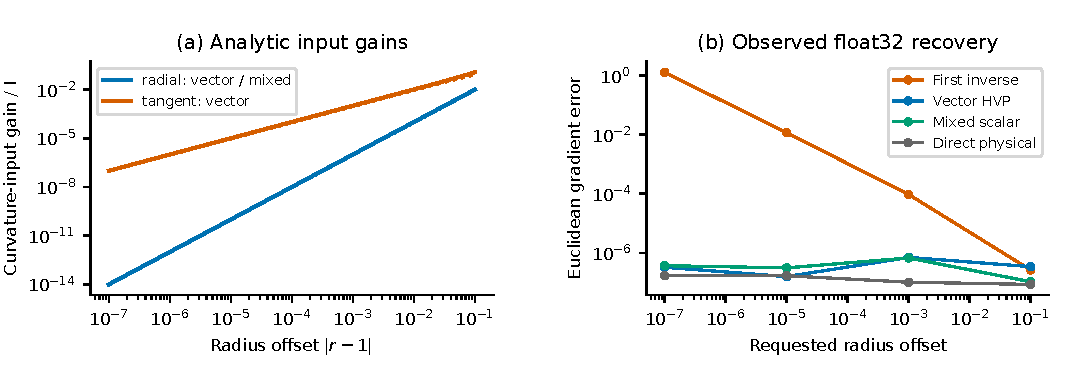
\includegraphics[width=.94\textwidth]{images/near_fold_information.pdf}
\caption{Theory and observed finite-precision error. (a) Vector-HVP curvature-input gains, normalized by intensity, on the inner and outer sheets. Mixed recovery uses only the radial coefficient. (b) Observed float32 gradient-recovery errors from the common-graph AD experiment at requested $I=1.2$, maximized over the two sheets at each requested radius offset. References are 80-digit physical gradients at the represented Stokes states. These are measured errors, not deterministic derivative-error envelopes. Prescribed-envelope experiments and the support-slack counterexample are specified in Supplementary Sections S4 and S8--S9.}
\label{fig:sensitivity}
\end{figure*}


\section{A quadratic gap-bound corollary}
\label{sec:gap}
Let $B\in\mathbb R^{m\times3}$ be a full-column-rank calibrated linear instrument, $y\in\mathbb R^m$ its observations, and $\Sigma\in\mathbb R^{m\times m}$ a fixed SPD observation covariance. Its data term can be written
\begin{equation}
 \begin{aligned}
 L(s)&=\tfrac12\|Bs-y\|_{\Sigma^{-1}}^2
       =\tfrac12\|s-z\|_W^2+c,\\
 W&=B^{\mathsf T}\Sigma^{-1}B,\qquad
 z=W^{-1}B^{\mathsf T}\Sigma^{-1}y,
 \end{aligned}
 \label{eq:calibrated}
\end{equation}
where $c$ is the additive least-squares residual independent of $s$. The generalized least-squares estimate $z$ can be unphysical. Define the constrained objective gap $\Delta_{\mathcal C}(s)=L(s)-\min_{u\in\mathcal C}L(u)$.

Set $M=W^{-1}$, $n=(-1,e)$, and $D_n=n^{\mathsf T}Mn$. For any mapped output $s_r=I(1,\phi e)$, the cone lies in the supporting half-space $H_e=\{u:n^{\mathsf T}u\leq0\}$ and
\begin{equation}
 n^{\mathsf T}(u-s_r)\leq\sigma_r,\quad
 \sigma_r=I(1-\phi)=\frac{I(r-1)^2}{1+r^2}.
 \label{eq:supportslack}
\end{equation}
\begin{corollary}[Quadratic gap bound from recovered gradients]
\label{cor:gap}
If $\|\widehat g-g\|_M\leq\eta$, then for any $\lambda\geq0$,
\begin{equation}
 \Delta_{\mathcal C}(s_r)\leq
 \tfrac12\bigl(\|\widehat g+\lambda n\|_M+\eta\bigr)^2
 +\lambda\sigma_r.
 \label{eq:nearcertificate}
\end{equation}
For an exact gradient, the minimizing multiplier is
\begin{equation}
 \lambda_r=\max\{0,-(n^{\mathsf T}Mg+\sigma_r)/D_n\}.
 \label{eq:nearmultiplier}
\end{equation}
\end{corollary}
\begin{proof}
For $u\in\mathcal C$ and $d=u-s_r$, complete the quadratic:
\begin{equation*}
 L(s_r)-L(u)\leq\tfrac12\|g+\lambda n\|_M^2+\lambda\sigma_r.
\end{equation*}
The triangle inequality gives \eqref{eq:nearcertificate}; minimizing the exact-gradient quadratic in $\lambda$ gives \eqref{eq:nearmultiplier}.
\end{proof}
At a fold $\sigma_r=0$. With $\widehat\lambda=\max\{0,-n^{\mathsf T}Mg/D_n\}$, define
\begin{equation}
 \mathcal B(s)=\tfrac12\|g+\widehat\lambda n\|_M^2.
 \label{eq:residualcertificate}
\end{equation}
This is exactly $L(s)-\min_{H_e}L$, the gap of the supporting-half-space relaxation. Its minimizer is $h_s=z-\widehat\lambda Mn$, so $\Delta_{\mathcal C}(s)=\mathcal B(s)$ if and only if $h_s\in\mathcal C$; strict convexity gives both directions. Supplementary Section S10 displays the two objective gaps. Alternatively, $g,W$ determine $z=s-W^{-1}g$, after which the original cone quadratic gives the exact gap. The half-space expression is the closed-form relaxation obtained by standard quadratic duality \cite{cvxbook}.

At an exact stationary fold, $g=\alpha n$ and the raw radial curvature in $w=(1+t)e$ is $\gamma_r=c_r=-I\alpha$. Nonnegative $\gamma_r$ gives the constrained optimum; negative $\gamma_r$ gives a strict saddle and gap at most $D_n\gamma_r^2/(2I^2)$. Supplementary Section S10 proves the classification and equality condition. A regular radial rescaling multiplies $\gamma_r$ by the squared coordinate Jacobian at stationarity. Its sign is invariant; the displayed coefficient uses $w=(1+t)e$.

Support slack remains necessary even with exact recovery; Supplementary Section S4 gives the positive-gap counterexample and Section S10 the relaxation geometry.





\section{Sequential initialization and boundary-restricted flow}
\label{sec:sequential}
A previous constrained estimate can be fully polarized. Every finite raw preimage of that nonzero boundary state has $r=1$. Exact optimization followed by a raw-coordinate lift can therefore put mass on the fold, even when the observations have a density. This is a conditional statement about a boundary estimate; it does not assert that a finite solver returns the exact fold. At a fold, the first-order obstruction is already described by smooth-lift theory \cite[Thm.~2.4]{lifts}. The following specialization explains what ordinary continuous flow does after such an initialization.

\begin{proposition}[Flow restricted to a Stokes fold]
\label{prop:restrictedflow}
Let $L(s)=\tfrac12\|s-z\|_W^2+c$, $W=\operatorname{diag}(1,1/2,1/2)$, and $z_I>\rho=\|z_p\|>0$. Use any $C^2$ bijective intensity coordinate onto $(0,\infty)$ with $I'\ne0$. For raw Euclidean gradient flow of $L\circ T_F$, the set $r=1$ is invariant. If $r(0)=1$ and $e(0)\ne-z_p/\rho$, then
\begin{equation}
 e(t)\longrightarrow z_p/\rho,\qquad
 I(t)\longrightarrow I_b=\frac{2z_I+\rho}{3}.
 \label{eq:foldflowlimit}
\end{equation}
The limiting state has gap $(z_I-\rho)^2/6$ and radial head curvature $-I_b(z_I-\rho)/3<0$.
\end{proposition}
\begin{proof}
Writing $a_r=2(1-r^2)/(1+r^2)^2$, the chain rule gives
\begin{equation}
 \frac{d r^2}{dt}=-2Ia_r w^{\mathsf T}g_p.
 \label{eq:radiusflow}
\end{equation}
Thus the smooth vector field is tangent to $r=1$, and uniqueness gives invariance. On that set, put $u=e^{\mathsf T}z_p/\rho$. Then
\begin{equation}
 \begin{aligned}
 \dot I&=-(I')^2(3I/2-z_I-\rho u/2),\\
 \dot u&=I\rho(1-u^2)/2.
 \end{aligned}
 \label{eq:restrictedflow}
\end{equation}
The intensity remains between the positive bounds $\min\{I(0),(2z_I-\rho)/3\}$ and $\max\{I(0),(2z_I+\rho)/3\}$. Hence $u\to1$ unless $u(0)=-1$. Scalar comparison in the first equation gives \eqref{eq:foldflowlimit}. Substitution into the quadratic objective and radial curvature gives the last assertion. Supplementary Section S16 details global existence and the antipodal exception.
\end{proof}

This is a property of continuous raw Euclidean flow. A plain gradient-descent step from the fold instead satisfies
\begin{equation}
 \|w-\eta\nabla_w(L\circ T_F)\|^2
 =1+\eta^2 I^2\|P_\perp g_p\|^2.
 \label{eq:discretefoldstep}
\end{equation}
It can leave the fold through a tangential update. Adam and quasi-Newton updates have different coordinate scalings and are not covered by invariance. The absolutely continuous random initialization and small fixed gradient step in \cite{lee} also differ from a boundary-derived initialization and finite solver termination. The proposition supplies a model-specific dynamical explanation; the numerical tests below evaluate discrete solvers directly.

\section{Numerical evaluation}
\label{sec:numerics}
Supplementary Sections S8--S13 document scalar, vector, and mixed recovery checks, controlled input errors, and 274 quadratic primal-dual records. They include three nonquadratic $C^2$ objectives and tests of the local-curvature correction. The main experiments evaluate finite-precision AD and shared-network fitting.

\subsection{Acquisition cost and finite-precision recovery}
We also evaluate all three routes and direct physical differentiation on the same eager PyTorch graph \cite{pytorch}. The objective is the quartic in Supplementary Section S9. The test uses one CPU thread on an Apple M4 Max, PyTorch 2.14.1, float32/float64, intensities $0.02,1.2$, and nine radii from $0.9$ to $1.1$, including offsets down to $10^{-7}$. Eighty-digit physical gradients at the represented Stokes states provide the error reference.

Table~\ref{tab:adcost} includes the cost of acquiring physical curvature in the corrected routes; Error32 and Error64 denote float32 and float64 gradient errors. This implementation obtains scalar curvatures by contracting vector HVPs. The largest float32 first-inverse error is $1.27$ at requested $I=1.2$, $r=0.9999999$ (represented radius $0.9999998808$), while the maximum vector and mixed errors are $7.07\times10^{-7}$ and $6.75\times10^{-7}$. This is error in recovering a physical gradient from rounded derivatives; it does not measure training failure. Direct differentiation has the smallest time and maximum-error entries in the table. The mixed route reduces the required curvature input to one scalar; these measurements distinguish that reduction from AD acquisition cost. Supplementary Section S14 gives timings on both sheets and at the fold, plus the warmup and batch protocol.
\begin{table}[!t]
\caption{Common-graph AD: median microseconds at $I=1.2$, $r=0.999$, float64; maximum Euclidean gradient error over the intensity/radius grid for each precision. Four exact-fold first-inverse cases are singular and omitted from error maxima.}
\label{tab:adcost}
\centering\small
\begin{tabular}{@{}lrrr@{}}\toprule
Route & $\mu$s & Error32 & Error64\\\midrule
Direct physical & 62.9 & $1.69\!\times\!10^{-7}$ & $5.00\!\times\!10^{-16}$\\
First inverse & 114.4 & $1.27\!\times\!10^{0}$ & $1.67\!\times\!10^{-9}$\\
Vector HVP & 274.5 & $7.07\!\times\!10^{-7}$ & $9.69\!\times\!10^{-16}$\\
Mixed scalar & 277.6 & $6.75\!\times\!10^{-7}$ & $9.99\!\times\!10^{-16}$\\
\bottomrule
\end{tabular}
\end{table}


\subsection{Shared-network fitting and fold incidence}
We fit noisy four-analyzer observations with a shared MLP: four input measurements, two width-32 hidden layers with SiLU activation $x/(1+e^{-x})$, and three head coordinates. The two $32\times32$ fields are the saved weak-polarization renderer reference and a synthetic field with DoLP $0.90$--$0.99$. Each run uses all 1,024 pixels, Gaussian analyzer noise with standard deviation $0.01$, float32 Adam, learning rate $0.003$, and 1,500 updates. Five seeds and two head initializations give 20 fixed runs. These are fixed fitting settings; Supplementary Section S15 specifies the initialization and diagnostics.

We evaluate each unaveraged pixel objective in independent head coordinates at updates $0,100,500,1000,1500$. A candidate requires $|r-1|\leq10^{-3}$ and normalized radial curvature $c_r/I^2<-10^{-7}$. The first threshold specifies a raw-radius neighborhood; the second excludes curvature values within $10^{-7}$ of zero. There are no such candidates at any saved checkpoint. Two high-DoLP pixels are within the radius threshold at update 500, both with nonnegative radial curvature. The closest final distances are $0.957$ for the renderer field and $0.0586$ for the high-DoLP field. The smaller radius thresholds $10^{-4}$ and $10^{-5}$ also give zero candidates.

Figure~\ref{fig:training} shows a fixed example, final radius distances, and learning curves. Independent-coordinate perturbations and a constructed stationary-fold control check the diagnostic and quadratic bound separately. The control is excluded from the incidence count. Twenty stored networks reproduce their saved predictions exactly; an independent AD check of 80 pixel Hessian contractions confirms the reported radial curvatures.

\begin{figure*}[!t]
\centering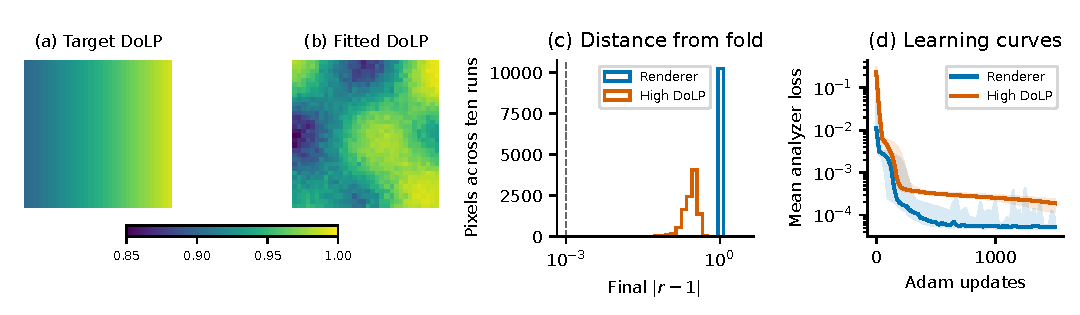
\includegraphics[width=\textwidth]{images/trained_fold_incidence.pdf}
\caption{Shared-network fitting in float32. (a)--(b) Target and fitted DoLP for the preselected high-DoLP field, standard initialization, seed 0. (c) Final radius-distance histograms over ten runs per field. The dashed line marks the $10^{-3}$ candidate radius threshold. (d) Median mean analyzer losses, with the full range across five seeds and two initializations. No saved checkpoint contains a near-fold negative-curvature candidate under the stated thresholds. These are single-field fits; the pixels are not independent experimental replications.}
\label{fig:training}
\end{figure*}


\subsection{Same-solver two-frame continuation}
\label{sec:warmexperiment}
We use 60 stored conditions: five noise seeds, three polarization angles $0,0.7,1.3$, two analyzer-noise standard deviations $0.001,0.01$, and next-frame DoLP $0.8,0.99$. The previous true DoLP is one and both true intensities are one. The same seed's noise is reused across conditions. These are dependent controlled conditions, not 60 independent scenes. Each solver estimates the previous frame from $(a,w)=(0,0.2,-0.1)$ with $I=\exp(a)$, then retains its raw coordinates for the next fit.

Before execution we fixed three angle changes $0,0.05,0.2$ radians, three solvers (BFGS, L-BFGS-B, and an exact-Hessian trust-region method), and gradient tolerances $10^{-4},10^{-6},10^{-8}$. This gives 1,620 continuations using the stored noise. A separate PyTorch LBFGS control uses genuine float32 and float64 tensors at tolerance $10^{-6}$, giving 360 continuations. A false success is solver acceptance with cone objective gap exceeding $10^{-6}$. PyTorch has no success flag, so its acceptance here means a finite native gradient infinity norm at most $10^{-6}$. Supplementary Section S17 specifies solver options and keeps nonacceptance separate from objective error.

We compare one unconditional radial restart with the same restart gated by $|r-1|\leq10^{-3}$ and $c_r/I^2<-10^{-7}$. The restart selects the lowest-loss point among offsets $\pm0.01$ and the current point, then reruns the same solver. A direct physical-gradient evaluation of Corollary~\ref{cor:gap}, including support slack, supplies a separate sufficient stopping test with bound threshold $10^{-6}$. A direct cone solution provides the reference objective.

\begin{table}[!t]
\caption{Zero angle change and tolerance $10^{-6}$. Every row uses the same 60 conditions. A pair is false successes / nonacceptances; the two categories are disjoint. PyTorch acceptance uses the operational gradient test.}
\label{tab:warm}
\centering\small
\begin{tabular}{@{}lrrr@{}}\toprule
Solver & Baseline & Always & Triggered\\\midrule
BFGS, float64 & 12 / 1 & 0 / 0 & 0 / 1\\
L-BFGS-B, float64 & 16 / 0 & 0 / 0 & 0 / 0\\
Trust region, float64 & 0 / 0 & 0 / 0 & 0 / 0\\
PyTorch LBFGS, float32 & 9 / 17 & 0 / 7 & 0 / 7\\
PyTorch LBFGS, float64 & 14 / 0 & 0 / 0 & 0 / 0\\\bottomrule
\end{tabular}
\end{table}

At tolerance $10^{-6}$, BFGS reproduces all 12 preliminary false-success condition IDs and the separate failure. L-BFGS-B and float64 PyTorch LBFGS also produce false successes (Table~\ref{tab:warm}); the effect is not limited to one implementation or float32 rounding. The trust-region arm has none. Changing angle by $0.05$ removes the SciPy false successes at this tolerance, while float64 PyTorch LBFGS retains one; changing by $0.2$ gives none in these arms. The float32 previous-frame fits have 22 nonacceptances among the 60 row references, retained in the comparison.

At zero angle change and tolerance $10^{-6}$, triggering detects all 28 SciPy false successes and no accurate accepted fit. BFGS uses 280 additional function/gradient pairs after triggering, against 479 after unconditional restarting; L-BFGS-B uses 320 against 496. Applying the radius test before curvature would require 17 and 21 full Hessian queries, respectively, plus endpoint diagnostic evaluations. For coverage analysis, the saved run evaluates curvature at every endpoint; Supplementary Section S17 separates that logging work from the required gated queries. These costs do not establish a wall-clock advantage. Unconditional restarting also repairs the nonfold BFGS failure, which the curvature gate misses.

The fixed gate is not a general stopping guarantee. At tolerance $10^{-4}$, the 540 SciPy continuations contain 68 false successes; triggering detects 14 and leaves 58 after restart, whereas unconditional restarting leaves 32. At zero angle change and tolerance $10^{-8}$, BFGS and L-BFGS-B each have eight false successes, reduced to zero by triggered restarting (Fig.~\ref{fig:warmaudit}(d)). Separately, BFGS has seven native failures, including six nonfinite terminal losses from exponential-intensity overflow; triggering retains all seven. Native failures and false successes are disjoint categories. Direct physical bounds falsely accept no inaccurate endpoint among the 1,620 SciPy continuations, and reject no endpoint whose finite gap is at most $10^{-6}$. These empirical checks accompany the analytic sufficient bound, not a universal exactness claim. The original 20 shared-MLP fits remain a separate experiment with no observed candidates.

\begin{figure*}[!t]
\centering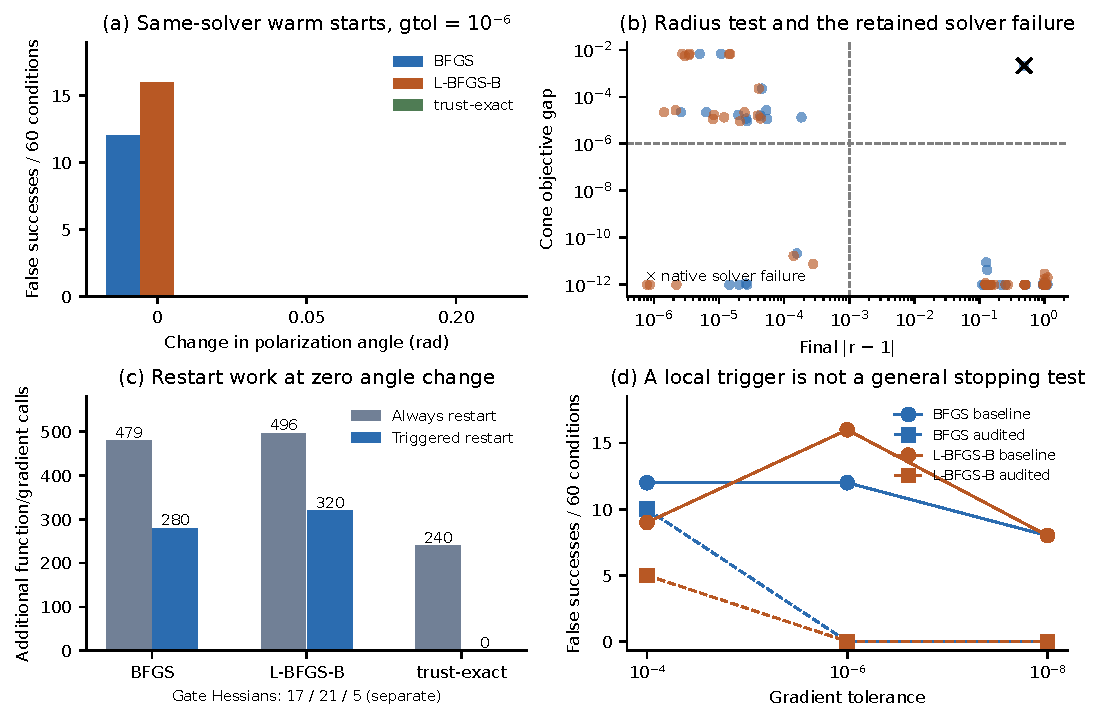
\includegraphics[width=\textwidth]{images/warm_start_audit.pdf}
\caption{Controlled two-frame stopping audit. The same 60 stored conditions are reused throughout. (a) False successes with tolerance $10^{-6}$. (b) Zero-angle-change endpoints for BFGS and L-BFGS-B; dashed lines mark the radius and gap thresholds. The cross is the nonfold BFGS failure. Displayed gaps below $10^{-12}$ and radius distances below $10^{-10}$ are clipped. (c) Additional restart function/gradient calls, including three trial pairs per restart. The separate Hessian counts are queries required after a radius guard; coverage logging evaluates every endpoint. (d) Zero-angle-change false-success counts across the fixed tolerances. Nonacceptances and nonfinite endpoints are retained in the records and are not plotted as false successes.}
\label{fig:warmaudit}
\end{figure*}

\subsection{A noisy physical-reflection sequence}
\label{sec:fresnel}
We generate a rocking air--dielectric interface from the Fresnel coefficients, with refractive index $1.5$ and incidence angle $\arctan(1.5)+18^{\circ}\cos(2\pi t/40)$ for $t=0,\ldots,40$. Unpolarized incident light gives normalized specular intensity one at Brewster's angle. Two polarization-orientation trajectories, three constant unpolarized background levels, two photon scales, and two seeds give 24 sequences and 984 frames per arm. Four ideal analyzer observations have independent Poisson shot noise and Gaussian read noise of standard deviation two electrons. We fit these observations with unweighted least squares.

Every solver/arm starts from $(0,0.2,-0.1)$ and inherits its own preceding raw endpoint. We use the existing $10^{-6}$ gradient tolerance, gap threshold, and local curvature gate, with at most one restart per frame. BFGS and L-BFGS-B report nine and seven inaccurate successes. Both curvature-triggered and physically audited branches have zero such endpoints, with seven interventions per solver; their corrections propagate through subsequent frames. On the uncorrected branches, the curvature gate detects all 16 false successes and flags no accurate accepted endpoint. The physical bound also rejects all 16. Both solvers have zero native failures in this grid. The simulation exhibits the fold mechanism under a specified physical noise model; direct physical auditing detects the same inaccurate endpoints. Supplementary Section S18 gives the complete protocol and alternative-map control.

\begin{figure*}[!t]
\centering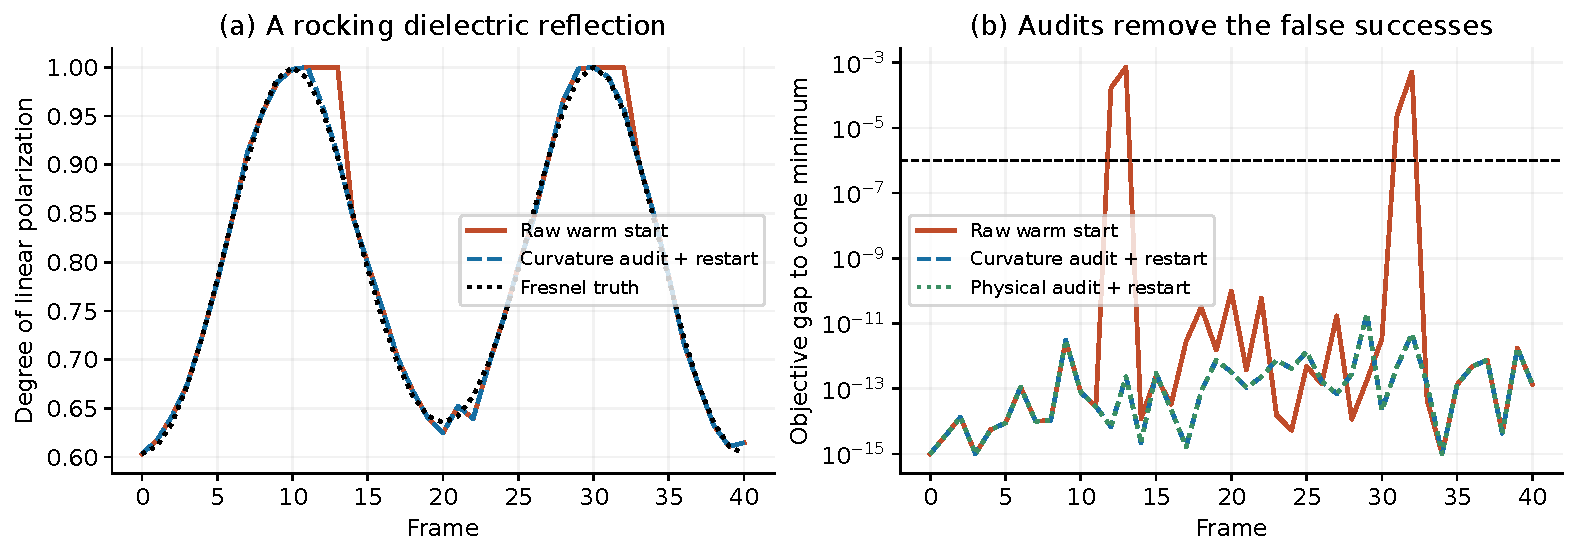
\includegraphics[width=.96\textwidth]{images/fresnel_sequence.pdf}
\caption{Fresnel-reflection continuation with shot and read noise. The displayed BFGS sequence is selected by the largest baseline objective gap in the fixed complete grid, rather than as a typical sequence. (a) Polarization estimate and physical truth. (b) Gap to the direct cone optimum; the dashed line is $10^{-6}$. Both audited branches overlap to plotting accuracy. Gaps below $10^{-15}$ are displayed at that floor. The complete grid has 984 frames per arm, with nine BFGS and seven L-BFGS-B false successes, versus zero in either audited branch.}
\label{fig:fresnel}
\end{figure*}

\subsection{Released polarization observations}
\label{sec:real}
We freeze small subsets of DeepSfP \cite{ba} and PolarNS/PolarBurstSR \cite{polarns} before optimization. DeepSfP contributes three indoor test objects and their four-angle observations. PolarNS contributes the lexicographically first object and scene mean/variance records, averaged over 10\,000 and 1\,017 captures. Those means are not treated as individual noisy frames. The first three released PolarBurstSR test crops contribute all 14 raw frames and four nominal color planes, unpacked with the authors' sensor layout.

For each static image, we select 128 seeded uniform eligible pixels and 64 pixels from an observed-high-DoLP stratum. For each burst color plane, a fixed $4\times4$ sensor grid is supplemented by eight high-DoLP positions selected using only the first frame. Finite, nonsaturated observations above a fixed relative intensity floor are eligible. The selections are reported separately in Supplementary Section S18; overlapping inputs and within-image/frame dependencies preclude a prevalence interpretation. Static samples follow a prescribed spatial scan. Burst samples follow fixed sensor coordinates without motion compensation, and are not asserted to follow one material point.

The reference is the cone optimum of the nominal four-analyzer quadratic. It measures optimization accuracy under that model; the available observations do not provide noise-free Stokes truth or a calibrated camera likelihood. Both solvers use $10^{-6}$ tolerance. Each arm carries its own state; a cold-start control resets intensity from the current observation and uses fixed polarization raw coordinates. The fixed protocol yields 576 DeepSfP, 384 PolarNS-mean, and 3\,682 burst entries per solver/arm, totaling 37\,136 fits across two solvers and four arms.

\begin{table*}[!t]
\caption{Released-data stopping audit. Every count pair is BFGS/L-BFGS-B. A false success is native acceptance with nominal quadratic gap above $10^{-6}$. Counts combine the separately reported sampling strata, not independent scenes. ``Detected'' and ``rejected'' refer to audits of the uncorrected warm-start endpoints. All native failure counts are zero.}
\label{tab:realdata}
\centering\small\renewcommand{\arraystretch}{1.15}
\begin{tabularx}{\textwidth}{@{}Xrrrrr@{}}\toprule
Subset & Entries & Cold false & Warm false & Local detected & Physical rejected\\\midrule
DeepSfP & 576 & 0/0 & 0/0 & 0/0 & 0/0\\
PolarNS means & 384 & 0/7 & 111/64 & 0/0 & 111/64\\
PolarBurstSR & 3\,682 & 0/7 & 16/104 & 0/0 & 16/104\\\bottomrule
\end{tabularx}
\end{table*}

Table~\ref{tab:realdata} shows inaccurate native successes in the PolarNS and burst subsets, while DeepSfP has none. None of the 295 uncorrected warm-start false successes satisfies the predeclared local fold gate, so curvature-triggered restarting leaves those counts unchanged. The physical bound rejects every inaccurate accepted endpoint. One physically audited radial restart leaves 68/64 native false successes in the PolarNS means and 16/99 in the bursts; their final bounds still reject them. The audit thus detects errors that a single radial restart leaves unresolved. On these observations, the physical stopping bound has broader coverage than the local fold gate. Figure~\ref{fig:realregimes} places them in the radius and gap-bound regimes.

An independent physical-coordinate SLSQP check of 29 selected reference minima has maximum loss discrepancy $1.31\times10^{-18}$. Independent float64 PyTorch AD audits all 309 cold/warm false successes and 32 control endpoints; maximum head-gradient, Hessian, and physical-gradient discrepancies are $7.77\times10^{-18}$, $8.89\times10^{-16}$, and $1.39\times10^{-17}$. No solver warning or native failure is removed. These checks assess the nominal objective and its derivatives. Aligned denoising, super-resolution, and surface-normal accuracy require separate evaluation.

\begin{figure*}[!t]
\centering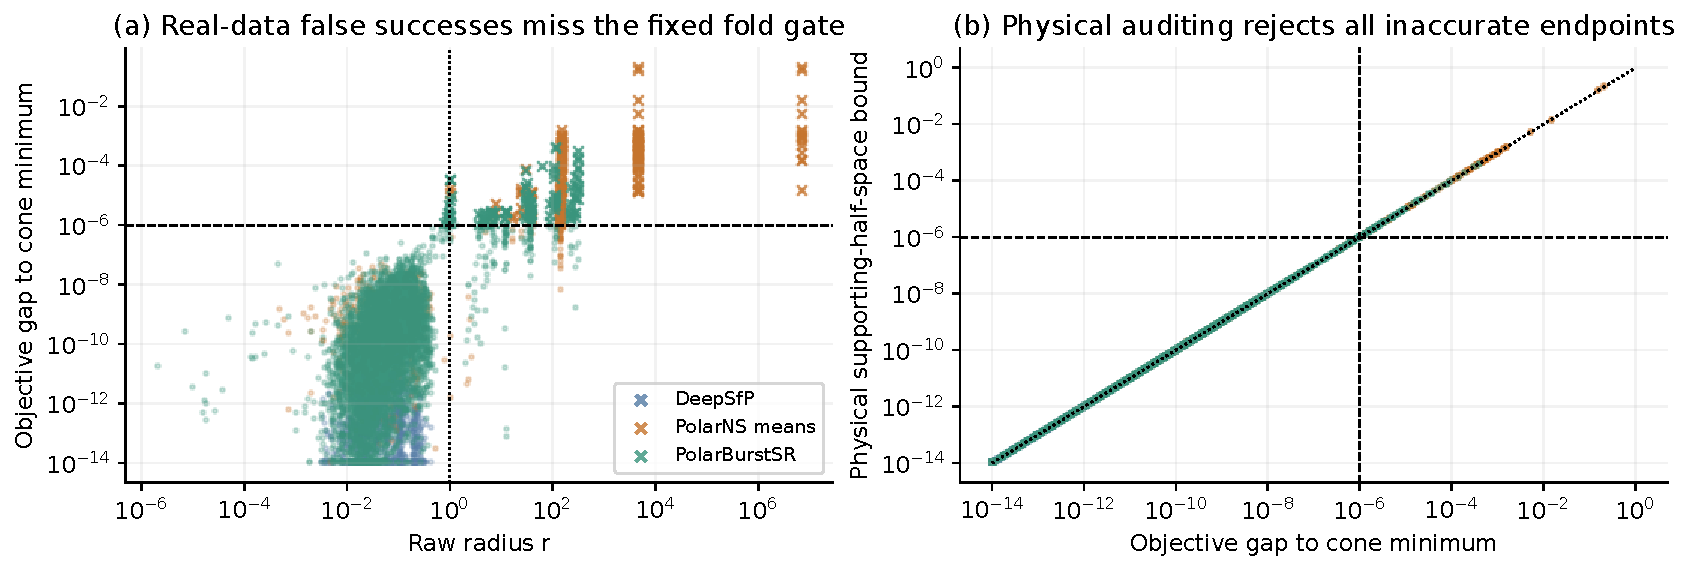
\includegraphics[width=.96\textwidth]{images/real_stopping_regimes.pdf}
\caption{All 9\,284 uncorrected real-data warm-start fits across two solvers. The subsets include uniform and enriched selections with repeated observations across distinct histories. (a) Objective gaps against raw radius. Crosses mark native false successes; the dotted line marks $r=1$ and the dashed line marks gap $10^{-6}$. None passes the fixed local fold gate. (b) Physical supporting-half-space bound against the reference gap; the dotted line is equality and dashed lines mark $10^{-6}$. The bound rejects all inaccurate endpoints. Values below $10^{-14}$ are displayed at that floor. The comparisons use float64 arithmetic, without outward-rounded certification.}
\label{fig:realregimes}
\end{figure*}

\subsection{Coordinate repair with physical stopping controls}
\label{sec:chartrepair}
The real-data failures motivate a follow-up on the same observations. We develop the repair rule after inspecting the previous audit, then freeze it before evaluation. The inputs, ordering, and thresholds are retained. Every arm carries its own preceding endpoint. Repeating the raw warm and cold branches reproduces all 18\,568 stored real-data endpoints exactly in raw coordinates.

For $r>1$, replacing $w$ by $C(w)=w/\|w\|^2$ preserves $F(w)$ and moves to the inner sheet. At fixed intensity and data, $\|\nabla_w\widetilde f(C(w))\|_2=r^2\|\nabla_w\widetilde f(w)\|_2$; the Jacobian condition number is unchanged. This relation follows from the paired preimages in Supplementary Section S6. A fresh solver invocation resets quasi-Newton memory. The fold and the dependence on intensity remain.

We compare applying this switch before every warm-start solve with a physically audited repair. On a bound rejection, the latter uses the existing radial trial rule if the local negative-curvature gate holds; otherwise it switches an outer endpoint and restarts once. Inner nonfold failures remain rejected. A control restarts once from the cold initialization instead. A guarded variant follows the coordinate repair with standard projected-gradient steps in physical coordinates when the bound still rejects. This fallback uses step one, at most 64 updates, and the same $10^{-6}$ bound threshold. No reference optimum initializes any iterative arm. A standalone physical projected-gradient solver and the direct cone solution are additional controls. Supplementary Section S19 specifies the algorithm and accounting.

\begin{table*}[!t]
\caption{Frozen coordinate-repair follow-up. Inaccurate means nominal gap above $10^{-6}$, irrespective of native or monitored acceptance. Count pairs are BFGS/L-BFGS-B, each with 4\,642 released-data entries and 984 Fresnel frames. Audited arms reject any remaining inaccurate outputs. Physical controls are single algorithms, without a head-solver pair. FG counts exclude separately recorded physical audits and Hessians.}
\label{tab:chartrepair}
\centering\small\renewcommand{\arraystretch}{1.12}
\begin{tabularx}{\textwidth}{@{}Xrrr@{}}\toprule
Strategy & Released inaccurate & Fresnel inaccurate & Released native FG pairs\\\midrule
Raw warm start & 127/168 & 9/7 & 92\,025/32\,235\\
Cold start & 0/14 & 0/0 & 97\,801/29\,468\\
Switch before each warm solve & 9/16 & 12/10 & 94\,974/32\,527\\
Audited cold restart & 0/2 & 0/0 & 95\,791/33\,232\\
Audited coordinate repair & 7/22 & 0/0 & 95\,640/33\,440\\
Coordinate repair with physical fallback & 0/0 & 0/0 & 95\,635/33\,245\\
Physical projected gradient & 0 & 0 & ---\\
Direct cone solution & 0 & 0 & ---\\\bottomrule
\end{tabularx}
\end{table*}

Table~\ref{tab:chartrepair} separates partial coordinate improvement from completed correction. Switching before each solve reduces released-data inaccurate endpoints from 295 to 25, but increases the Fresnel count from 16 to 22. The audited coordinate arm leaves 29 inaccurate released-data endpoints, all rejected. Adding physical fallback leaves none: BFGS and L-BFGS-B require respectively two and 15 fallback calls, with three and 22 projected updates in total. There are 4\,663/4\,704 physical-gradient queries in those guarded branches, including stopping audits. No real-data repair invokes the local curvature gate. In the Fresnel grid, each guarded solver uses seven full head-Hessian queries and 21 trial FG evaluations; neither requires physical fallback.

A separate paired-endpoint audit applies the repair to the same 9\,284 historical warm endpoints, rather than changed continuation histories. Coordinate repair leaves 7/39 of the original 127/168 inaccurate endpoints; physical fallback removes those remaining 46. Audited cold restarting leaves 0/5. Thus the coordinate-only step corrects 249 of the 295 original failures, while full correction depends on the physical fallback. Independent PyTorch checks cover all 295 historical false successes and 32 controls; the largest output-preservation and gradient-transformation discrepancies are $1.74\times10^{-18}$ and $7.78\times10^{-16}$.

The physical controls are substantially cheaper in this implementation. Across 4\,642 released entries, standalone projected gradient uses 9\,575 updates and 14\,217 physical-gradient queries, with no inaccurate or rejected outputs. Its observed time is 0.203 s, versus 4.64/1.35 s for the guarded head solvers and 0.0219 s for the direct cone solution. These timings describe one CPU pass in the stated implementation. Coordinate repair provides a partial remedy for existing head-based fits; the direct physical methods are more economical for this quadratic. All released-data repairs in this follow-up use first derivatives.



\section{Finite-tolerance stopping guarantees}
\label{sec:stoppingguarantees}
The recovery formulas identify the physical gradient from head derivatives. For stopping, we also need a tolerance that controls the objective gap. For strongly convex physical objectives, a lower test on one radial curvature near the fold provides such a bound.

\subsection{Relation to approximate-lift results}
Approximate second-order transfer is established for squared-variable formulations \cite[Thm.~3.6 and Cor.~3.7]{dingwright}. Local gap control through the Kurdyka--\L{}ojasiewicz (KL) exponent is also established for Hadamard difference parametrizations \cite[Thm.~3.11 and Rem.~3.12]{ouyang}. In particular, a KL exponent $3/4$ leads to a gradient-to-gap power $4/3$. Table~\ref{tab:stoppingprior} places the Stokes result in this framework. It gives explicit constants over the whole inner sheet with bounded intensity, uses one radial lower-curvature test, and accommodates supplied derivative-error budgets. Its domain is specified by evaluated coordinates and model bounds, independently of the distance to an optimum or nondegeneracy at that optimum.

\begin{table*}[!t]
\caption{Comparison for finite-tolerance stopping. PDF theorem locators for the three external preprints use arXiv:2310.01784v2, 2402.00377v2, and 2112.05273v2, respectively. The columns identify the feasible sets, assumptions, and conclusions relevant to the Stokes specialization.}
\label{tab:stoppingprior}
\centering\small\renewcommand{\arraystretch}{1.12}
\begin{tabularx}{\textwidth}{@{}p{.24\textwidth}p{.37\textwidth}X@{}}\toprule
Prior result & Established guarantee & Present specialization\\\midrule
Ding--Wright, Thm.~3.6, Cor.~3.7 \cite{dingwright} & Approximate squared-slack second-order conditions transfer to approximate weak second-order conditions, with active-Jacobian rank and conditioning dependencies. & Direct gap bound for strongly convex Stokes objectives, with one radial curvature and explicit constants.\\
Ouyang \emph{et al.}, Thm.~3.11, Rem.~3.12 \cite{ouyang} & Local KL exponents for Hadamard difference models; exponent $3/4$ occurs without strict complementarity under error-bound assumptions. & Uniform derivative-tolerance bound on a stated chart domain; $4/3$ is consistent with this known exponent.\\
Li \emph{et al.}, Thm.~5, Lem.~6.1 \cite{hadamard} & Algorithmic gap guarantee under strict-saddle and nondegeneracy assumptions; compactness gives qualitative approximate-to-exact proximity. & Deterministic stopping implication without those assumptions, for the narrower strongly convex physical class.\\\bottomrule
\end{tabularx}
\end{table*}

\subsection{One radial test and a uniform gap bound}
Write $\Delta(s)=f(s)-\min_{u\in\mathcal C}f(u)$ for the objective gap and $x_+=\max\{x,0\}$ for the positive part. At the evaluated point, retain $b=\partial_a\widetilde f/I'$ and $j=\nabla_w\widetilde f$. For $r>0$, set $c_r=e^{\mathsf T}\nabla^2_{ww}\widetilde f\,e$. The following gradient tolerance is normalized in physical units; Supplementary Section S20 gives the conversion from a native solver tolerance.

\begin{theorem}[Uniform stopping on the inner Stokes sheet]
\label{thm:uniformstopping}
Let $f:\mathbb R^3\to\mathbb R$ be $C^2$ and $\mu$-strongly convex, $\mu>0$, and fix $L\ge\mu$. At $s=T_F(a,w)$, suppose $0<I\le\overline I$, $0\le r\le1$, and
\begin{equation}
 |b|\le\varepsilon,\qquad \|j\|_2/I\le\varepsilon.
 \label{eq:normalizedstop}
\end{equation}
When $r\ge1/2$, additionally suppose
\begin{equation}
 e^{\mathsf T}H_{pp}(s)e\le L,\qquad c_r\ge-I\nu,
 \quad L\ge\mu,\quad \nu\ge0.
 \label{eq:radialstop}
\end{equation}
No curvature observation is required at $r<1/2$. Put $K_0=\overline I L$ and assume $\varepsilon\le K_0/8$. Then
\begin{equation}
 \boxed{\ f(s)-\min_{u\in\mathcal C}f(u)
 \le \frac{52K_0^{2/3}}{\mu}\varepsilon^{4/3}
       +\frac{3}{\mu}\nu^2.\ }
 \label{eq:uniformstopgap}
\end{equation}
The coefficient 52 is conservative; the two tolerance orders are sharp.
\end{theorem}
\begin{proof}
Write $g_p=me+u$, $u\perp e$, and $\delta=1-r$. Then $g_I=b-\phi m$, $|a_rm|\le\varepsilon$, and $\|u\|\le\varepsilon/t_r$. Strong convexity and the supporting inequality give, for every $\lambda\ge0$,
\begin{equation}
 \Delta(s)\le\frac{\|g+\lambda n\|_2^2}{2\mu}
                  +\lambda I(1-\phi),\quad n=(-1,e).
 \label{eq:strongstopdual}
\end{equation}
For any $0<h\le1/2$, $\delta\ge h$ implies $a_r\ge\delta$ and hence $\Delta(s)\le3\varepsilon^2/(\mu h^2)$. If $\delta<h$, then $1\le|\kappa_r|$, $a_r\le2\delta$, and $1-\phi\le\delta^2$. The radial identity $c_r/I=Ia_r^2 e^{\mathsf T}H_{pp}e+\kappa_r m$ yields
\begin{equation}
 m_+\le\nu+4K_0\delta^2.
 \label{eq:positivegradientbound}
\end{equation}
Choose $\lambda=(-m)_+$. For $m<0$, use $|m|(1-\phi)\le\varepsilon\delta$; for $m\ge0$, use \eqref{eq:positivegradientbound}. The two cases give
\begin{equation}
 \Delta(s)\le\frac{5\varepsilon^2+6\nu^2+96K_0^2h^4}{2\mu}
                  +\overline I\varepsilon h.
 \label{eq:bandstopgap}
\end{equation}
Set $h=(\varepsilon/K_0)^{1/3}$ and use $L\ge\mu$ to obtain \eqref{eq:uniformstopgap}. The zero-tolerance case follows separately or by taking a limit. At $r=0$, $DF=2\operatorname{Id}_2$ gives the first-order bound directly. Supplementary Section S20 gives all inequalities and a tighter pointwise certificate.
\end{proof}

\subsection{Input errors and a target stopping rule}
Suppose supplied $\widehat b,\widehat j,\widehat c_r$ have valid error budgets $E_b,E_j,E_c$:
\begin{equation}
 |\widehat b-b|\le E_b,\quad\|\widehat j-j\|\le E_j,
 \quad|\widehat c_r-c_r|\le E_c.
 \label{eq:stopinputerrors}
\end{equation}
With exact evaluated geometry, sufficient tolerance values are
\begin{equation}
 \begin{aligned}
 \varepsilon&=\max\{ |\widehat b|+E_b,
                         (\|\widehat j\|+E_j)/I\},\\
 \nu&=\max\{0,(-\widehat c_r+E_c)/I\}.
 \end{aligned}
 \label{eq:stopinflation}
\end{equation}
The triangle inequality gives this inflation. Applying it requires valid budgets and justified bounds $\mu,L,\overline I$ for the objective being optimized. Numerical certification would additionally require validated rounding-error bounds; the measured float32/float64 discrepancies alone are insufficient. Equation~\eqref{eq:stopinputerrors} assumes exact evaluated geometry and a fixed instrument model.

For a desired objective gap $\tau>0$, one explicit sufficient rule is
\begin{equation}
 \begin{aligned}
 \varepsilon&\le\min\!\left\{K_0/8,
            \left(\frac{\mu\tau}{104K_0^{2/3}}\right)^{3/4}\right\},\\
 \nu&\le\sqrt{\mu\tau/6}.
 \end{aligned}
 \label{eq:targetstop}
\end{equation}
Theorem~\ref{thm:uniformstopping} then gives $\Delta(s)\le\tau$. A raw gradient tolerance requires conversion through $I$ and $I'$; without positive lower bounds on $I$ and $|I'|$ it cannot uniformly imply \eqref{eq:normalizedstop}. The rule certifies the gap at any point satisfying these conditions. The number of iterations needed to reach them depends on the optimizer.

\subsection{Sharp orders and necessary restrictions}
The $4/3$ order cannot be replaced uniformly by a larger power. For the fixed objective $f(s)=\tfrac12\|s-(1,e)\|^2$, take $r\uparrow1$ and $I=(1+\phi)/(1+\phi^2)$. Then $b=0$, $c_r\ge0$, and, with $\delta=1-r$,
\begin{equation}
 \varepsilon\sim\delta^3/4,\qquad
 \Delta(s)\sim\delta^4/16,\qquad
 \Delta/\varepsilon^{4/3}\to2^{-4/3}.
 \label{eq:stopsharpfirst}
\end{equation}
For the curvature order, the fold family in Fig.~\ref{fig:principle}, with Euclidean metric and $g=\alpha(-1,e)$, $\alpha>0$, has $\varepsilon=0$, $\nu=\alpha$ and exact gap $\alpha^2$. Thus a larger power than $\nu^2$ also fails. Both orders are therefore sharp within the stated objective class.

Curvature cannot be omitted at the fold: the same family has zero first derivatives and positive gap. The inner-sheet restriction is also necessary for this uniform implication. On an unbounded outer sheet, the quadratic centered at $(1,1/2,0)$ admits states with both normalized first derivatives and negative radial curvature tending to zero while the gap tends to $1/8$. With exponential intensity, raw first- and second-order tests also tend to zero as $I\downarrow0$ for the quadratic centered at $(1,0,0)$, while its gap tends to $1/2$. Section S20 supplies the constructions. Moving inward preserves the physical output but requires recomputing derivative tests there.

\subsection{Numerical verification}
A fixed check set contains 576 quadratic and 24 strongly convex quartic objectives with three supplied derivative-error budgets, giving 1\,800 checks. The uniform small-tolerance condition applies in 1\,431. The largest computed gap above a bound is $1.24\times10^{-14}$; the independent SLSQP references have feasibility residual as low as $-9.64\times10^{-14}$. All 600 reference solves return success. Independent PyTorch differentiation gives maximum $b$, $j$, and $c_r$ discrepancies $1.78\times10^{-15}$, $5.33\times10^{-15}$, and $1.43\times10^{-14}$. Ninety-digit decimal examples check the sharp-order limits and the counterexamples.

On the existing 9\,284 real-data warm endpoints, we switch outer coordinates inward and recompute derivatives, without running another solver. The pointwise certificate in Section S20 accepts 8\,861 endpoints at nominal gap $10^{-6}$, rejects all 295 historical false successes, and additionally rejects 128 accurate endpoints. The coarse uniform bound alone accepts 980. This retrospective calculation checks the formula's coverage using zero supplied error budgets in float64 and a full analytic head Hessian at every endpoint. Its cost includes these Hessians. Direct physical auditing and the direct solvers in Section~\ref{sec:chartrepair} provide the practical cost comparison.

Section S21 adds outward evaluation of the nominal quadratic bound, including exponential intensity, geometry, and derivative arithmetic. At 128 fractional bits, it certifies gap at most $10^{-6}$ for the same 8\,861 endpoints and rejects all 295 inaccurate endpoints; 128 accurate endpoints remain rejected. It uses 52 scalar curvature evaluations and forms no full head Hessian. The complete pass takes 7.32 s. Decisions agree at 64--256 bits; 32 bits leave three additional accurate endpoints inconclusive. The accompanying standard-library implementation returns an integer-enclosed bound or an explicit inconclusive result.


\section{Discussion}
At the fold, the physical-gradient ambiguity has dimension one, and one signed radial curvature resolves it without knowledge of the physical Hessian. Away from the fold, full first derivatives suffice. Additional physical-curvature input is needed only for the restricted mixed or vector observation sets. The scalar and vector formulas therefore solve different observation problems.

The choice of route also changes sensitivity. The mixed route has only a quadratic radial curvature-input gain; the vector route adds a first-order tangential gain. Both retain derivative-error coefficients proportional to $1/I$. Radius, direction, and intensity are computed from the head coordinates. The input-error formulas hold at that evaluated geometry; coordinate perturbations define a separate sensitivity problem.

The real-data endpoints illustrate why small head derivatives can coexist with a substantial physical objective gap away from the fold. Polarization-gradient inversion in \eqref{eq:firstinverse} includes the gain $1/(I\min\{|a_r|,t_r\})$. It grows at the fold, at small intensity, and as $r^2/(2I)$ on the large-radius outer sheet. Thus avoiding the fixed fold neighborhood does not ensure reliable first-order stopping. The released-data audit contains outer-sheet radii above $10^2$, while the DeepSfP subset remains well inside the fold. The same inverse therefore explains several regimes in which the local fold gate has different coverage.

The stopping theorem applies to strongly convex physical objectives on the bounded-intensity inner sheet. Within that domain, one radial lower-curvature test suffices; a full positive-semidefinite head Hessian is unnecessary. Strong convexity turns the derivative conditions into a global objective-gap bound. The pointwise expression is less conservative than the uniform thresholds, yet still rejects 128 accurate historical endpoints. The outward implementation in Section S21 encloses intensity, coordinate geometry, and derivative arithmetic for the nominal ideal quadratic. It verifies the same acceptance decisions at 64--256 fractional bits. Extending this implementation to uncertain instrument models, and designing an optimizer that reaches the sufficient conditions efficiently, remain separate tasks.

An endpoint audit can proceed in four steps: (i)~inspect $r,I,I'$ and the inverse gains before applying a near-fold radius gate; (ii)~at the exact fold, use one signed radial curvature for recovery and stationary-fold classification in the calibrated quadratic; at finite offsets, follow Table~\ref{tab:contract}; (iii)~use a calibrated $W\succ0$ and a valid gradient-error bound in Corollary~\ref{cor:gap}, retaining the support slack, or apply Theorem~\ref{thm:uniformstopping} after checking its assumptions; accept when a valid gap upper bound meets the target, and continue assessment otherwise; (iv)~when a physical-gradient oracle is available, evaluate the applicable bound directly. For the tested nominal quadratics, the direct cone solution and physical projected gradient in Section~\ref{sec:chartrepair} are cheaper routes to an accepted endpoint. Small or uncertain curvature can leave the derivative-based decision inconclusive. Coordinate repair and physical fallback illustrate subsequent actions on rejected endpoints.

The shared-network experiment supplies a further boundary on the empirical evidence: its 20 fits contain no saved near-fold negative-curvature candidates. Extending the analysis from independent head coordinates to shared network parameters requires a separate error model.

\section{Conclusion}
One signed radial curvature restores the physical-gradient component lost at the rational Stokes fold. Mixed and vector inverses extend recovery with explicit error gains. For strongly convex physical objectives with bounded intensity, one radial lower-curvature test and normalized head derivatives give an inner-sheet gap bound with sharp orders $\varepsilon^{4/3}+\nu^2$. Valid error budgets turn this bound into sufficient stopping thresholds; an outward interval implementation supplies a numerical certificate for the nominal ideal quadratic. The experiments show where these derivative tests help and where direct physical methods are preferable: the local gate detects controlled fold failures, coordinate switching repairs part of the released-data failures, and standard physical fallback completes correction. Together, the recovery formulas, stopping bounds, and counterexamples describe the information needed to assess convergence through this folded parametrization.

\section*{Acknowledgment}
OpenAI Codex~\cite{codex} was used to draft and revise text in the abstract, Sections I--X, and Supplementary Material, and to assist with mathematical derivations and preparation of experimental and verification code. The authors take responsibility for the content.

\section*{Data and code availability}
Code, numerical records, figure generators, and TeX sources are available at \url{https://github.com/usamihiroyasu/stokes-gradient-recovery}. The released-observation audit records exact archive members, byte ranges, checksums, selected coordinates, and observations; full source images remain available from the original providers \cite{ba,polarns}. Reproduction commands and file hashes are in \nolinkurl{README.md} and \nolinkurl{MANIFEST.sha256}.

\FloatBarrier
\begin{thebibliography}{14}
\bibitem{hu} H. Hu, G. Anna, and F. Goudail, ``On the performance of the physicality-constrained maximum-likelihood estimation of Stokes vector,'' \emph{Appl. Opt.}, vol. 52, no. 27, pp. 6636--6644, 2013, doi: \href{https://doi.org/10.1364/AO.52.006636}{\nolinkurl{10.1364/AO.52.006636}}.

\bibitem{spc} S. Song and T. Mu, ``Stokes physical constraint method for improving polarization imaging-based vision task,'' \emph{Opt. Laser Technol.}, vol. 192, Part A, Art. no. 113408, 2025, doi: \href{https://doi.org/10.1016/j.optlastec.2025.113408}{\nolinkurl{10.1016/j.optlastec.2025.113408}}.

\bibitem{psara} J. Birdi, A. Repetti, and Y. Wiaux, ``Sparse interferometric Stokes imaging under the polarization constraint (Polarized SARA),'' \emph{Mon. Not. R. Astron. Soc.}, vol. 478, no. 4, pp. 4442--4463, 2018, doi: \href{https://doi.org/10.1093/mnras/sty1182}{\nolinkurl{10.1093/mnras/sty1182}}.

\bibitem{ba} Y. Ba \emph{et al.}, ``Deep shape from polarization,'' in \emph{Proc. Eur. Conf. Comput. Vis.}, 2020. [Online]. Available: \url{https://www.ecva.net/papers/eccv_2020/papers_ECCV/html/4676_ECCV_2020_paper.php}

\bibitem{pandora} A. Dave, Y. Zhao, and A. Veeraraghavan, ``PANDORA: Polarization-aided neural decomposition of radiance,'' in \emph{Proc. Eur. Conf. Comput. Vis.}, 2022. [Online]. Available: \url{https://akshatdave.github.io/pandora/}

\bibitem{polarns} I. Hwang, K. Choi, H. Ha, and M. H. Kim, ``Benchmarking burst super-resolution for polarization images: Noise dataset and analysis,'' in \emph{Proc. IEEE/CVF Int. Conf. Comput. Vis.}, pp. 24899--24909, 2025. [Online]. Available: \url{https://openaccess.thecvf.com/content/ICCV2025/html/Hwang_Benchmarking_Burst_Super-Resolution_for_Polarization_Images_Noise_Dataset_and_Analysis_ICCV_2025_paper.html}

\bibitem{optnet} B. Amos and J. Z. Kolter, ``OptNet: Differentiable optimization as a layer in neural networks,'' in \emph{Proc. 34th Int. Conf. Mach. Learn.}, PMLR, vol. 70, pp. 136--145, 2017. [Online]. Available: \url{https://proceedings.mlr.press/v70/amos17a.html}

\bibitem{cvxlayers} A. Agrawal, B. Amos, S. Barratt, S. Boyd, S. Diamond, and J. Z. Kolter, ``Differentiable convex optimization layers,'' in \emph{Adv. Neural Inf. Process. Syst.}, vol. 32, 2019. [Online]. Available: \url{https://papers.neurips.cc/paper_files/paper/2019/hash/9ce3c52fc54362e22053399d3181c638-Abstract.html}

\bibitem{hardnet} Y. Min and N. Azizan, ``HardNet: Hard-constrained neural networks with universal approximation guarantees,'' \emph{arXiv:2410.10807v4}, revised Oct. 19, 2025, first submitted 2024. [Online]. Available: \url{https://arxiv.org/abs/2410.10807v4}

\bibitem{gcopter} Z. Wang, X. Zhou, C. Xu, and F. Gao, ``Geometrically constrained trajectory optimization for multicopters,'' \emph{IEEE Trans. Robot.}, vol. 38, no. 5, pp. 3259--3278, 2022, doi: \href{https://doi.org/10.1109/TRO.2022.3160022}{\nolinkurl{10.1109/TRO.2022.3160022}}.

\bibitem{lifts} E. Levin, J. Kileel, and N. Boumal, ``The effect of smooth parametrizations on nonconvex optimization landscapes,'' \emph{Math. Program.}, vol. 209, pp. 63--111, 2025, doi: \href{https://doi.org/10.1007/s10107-024-02058-3}{\nolinkurl{10.1007/s10107-024-02058-3}}. Theorem locators use \href{https://arxiv.org/abs/2207.03512v5}{arXiv:2207.03512v5}.

\bibitem{hadamard} Q. Li, D. McKenzie, and W. Yin, ``From the simplex to the sphere: Faster constrained optimization using the Hadamard parametrization,'' \emph{Information and Inference}, vol. 12, no. 3, pp. 1898--1937, 2023, doi: \href{https://doi.org/10.1093/imaiai/iaad017}{\nolinkurl{10.1093/imaiai/iaad017}}. Theorem locators use \href{https://arxiv.org/abs/2112.05273v2}{arXiv:2112.05273v2}.

\bibitem{cvxbook} S. Boyd and L. Vandenberghe, \emph{Convex Optimization}. Cambridge, U.K.: Cambridge University Press, 2004, ch. 5. [Online]. Available: \url{https://web.stanford.edu/~boyd/cvxbook/}

\bibitem{pytorch}
A. Paszke \emph{et al.}, ``PyTorch: An imperative style, high-performance deep learning library,'' in \emph{Adv. Neural Inf. Process. Syst.}, vol.~32, 2019.
\bibitem{lee} J. D. Lee, M. Simchowitz, M. I. Jordan, and B. Recht, ``Gradient descent only converges to minimizers,'' in \emph{Proc. 29th Conf. Learning Theory}, vol. 49, pp. 1246--1257, 2016. [Online]. Available: \url{https://proceedings.mlr.press/v49/lee16.html}

\bibitem{dingwright} L. Ding and S. J. Wright, ``On squared-variable formulations,'' \emph{SIAM J. Optim.}, vol. 35, no. 4, pp. 2265--2293, 2025, doi: \href{https://doi.org/10.1137/23M1608343}{\nolinkurl{10.1137/23M1608343}}. Theorem locators use \href{https://arxiv.org/abs/2310.01784v2}{arXiv:2310.01784v2}.

\bibitem{ouyang} W. Ouyang, Y. Liu, T. K. Pong, and H. Wang, ``Kurdyka--\L{}ojasiewicz exponent via Hadamard parametrization,'' \emph{SIAM J. Optim.}, vol. 35, no. 1, pp. 62--91, 2025, doi: \href{https://doi.org/10.1137/24M1636186}{\nolinkurl{10.1137/24M1636186}}. Theorem locators use \href{https://arxiv.org/abs/2402.00377v2}{arXiv:2402.00377v2}.

\bibitem{codex} OpenAI, ``Codex.'' Accessed: Oct. 22, 2026. [Online]. Available: \url{https://openai.com/codex/}

\end{thebibliography}

\end{document}
